\begin{center}
    \textbf{Geração 60}
\end{center}

\begin{figure}[h]
    \centering
    \label{fig:geracaoXX}
    
    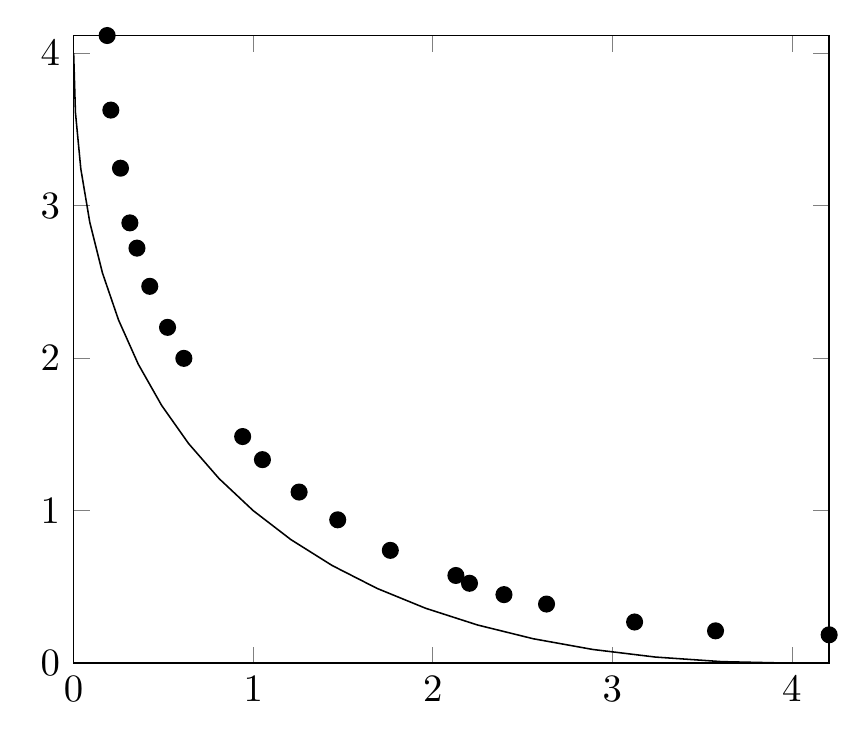
\begin{tikzpicture}[scale=1.4]
        \begin{axis}[enlargelimits=false]
            \addplot [] coordinates {
                (0.000000,4.000000) (0.010000,3.610000) (0.040000,3.240000) (0.090000,2.890000) (0.160000,2.560000) (0.250000,2.250000) (0.360000,1.960000) (0.490000,1.690000) (0.640000,1.440000) (0.810000,1.210000) (1.000000,1.000000) (1.210000,0.810000) (1.440000,0.640000) (1.690000,0.490000) (1.960000,0.360000) (2.250000,0.250000) (2.560000,0.160000) (2.890000,0.090000) (3.240000,0.040000) (3.610000,0.010000) (4.000000,0.000000) 
            };
            
            \addplot [only marks] coordinates {
                (4.207380,0.185885) (0.186601,4.115023) (0.941196,1.485769) (0.613711,1.998401) (0.260899,3.245099) (3.574649,0.211924) (1.255567,1.121880) (3.123972,0.269869) (0.423875,2.470665) (1.763537,0.739618) (0.207033,3.626073) (2.633520,0.387560) (2.128749,0.574927) (0.522969,2.201617) (0.352627,2.721092) (1.470639,0.939838) (2.396409,0.449372) (0.313111,2.886601) (1.051384,1.334385) (2.204450,0.523775) 
            };
        \end{axis}
    \end{tikzpicture}
\end{figure}